\chapter{Fermi and Bose Particles}
    \section{Fermions}    
        Consider the grand partition function for fermions and bosons. We start with the fermions. We will look at a system of non-interacting fermions that populate single energy states $\phi_v{k}(\v{r})$ with energy $\varepsilon(\v{k})=\varepsilon(k)$. An important distinction that we have to keep in mind is that $\varepsilon(k)$ represents the energies of the single particles while $E_i$ represents the energies of multiple-particles. Since we either have no occupence or a single occupence for a given $\v{k}$, the grand partition function is
        \begin{equation}
            \Theta(\v{k}) = \sum_ie^{-\beta(E_i-\mu)} = 1+e^{-\beta(\varepsilon(k)-\mu)}.
        \end{equation}
        This gives the grand potential as: $\Phi_G = -k_BT\ln\lrp{1+e^{-\beta(\varepsilon-\mu)}}$. \\
        Looking at a single $\v{k}$, the average number of particles in this state $\varepsilon(k)$ is
        \begin{equation}
            n(\v{k}) = -\frac{\del \Phi_G}{\del \mu} = -k_BT\frac{\beta e^{-\beta(\varepsilon-\mu)}}{1+e^{-\beta(\varepsilon-\mu)}} = \frac{1}{e^{\beta(\varepsilon(k)-\mu)}+1}.
        \end{equation}
        This is the \textbf{Fermi-Dirac Distribution}. Let us now look at the limits. Here, we need to remember that the chemical potential also depends on the temperature. As $T\to\infty$, $\mu\to-\infty$. Therefore, at high temperatures, $-\mu/k_BT>>1$ and we get $ n(\v{k}) \approx e^{-\beta(\varepsilon(k)-\mu)}$. Since the chemical potential is a positive quantity, at low temperatures, the exponent goes to zero and we get $n(\v{k})=1$. At absolute zero, the chemical potential equals the \textbf{Fermi energy}, which is the energy of the highest occupied state.
        \begin{figure}[h!]
            \centering
            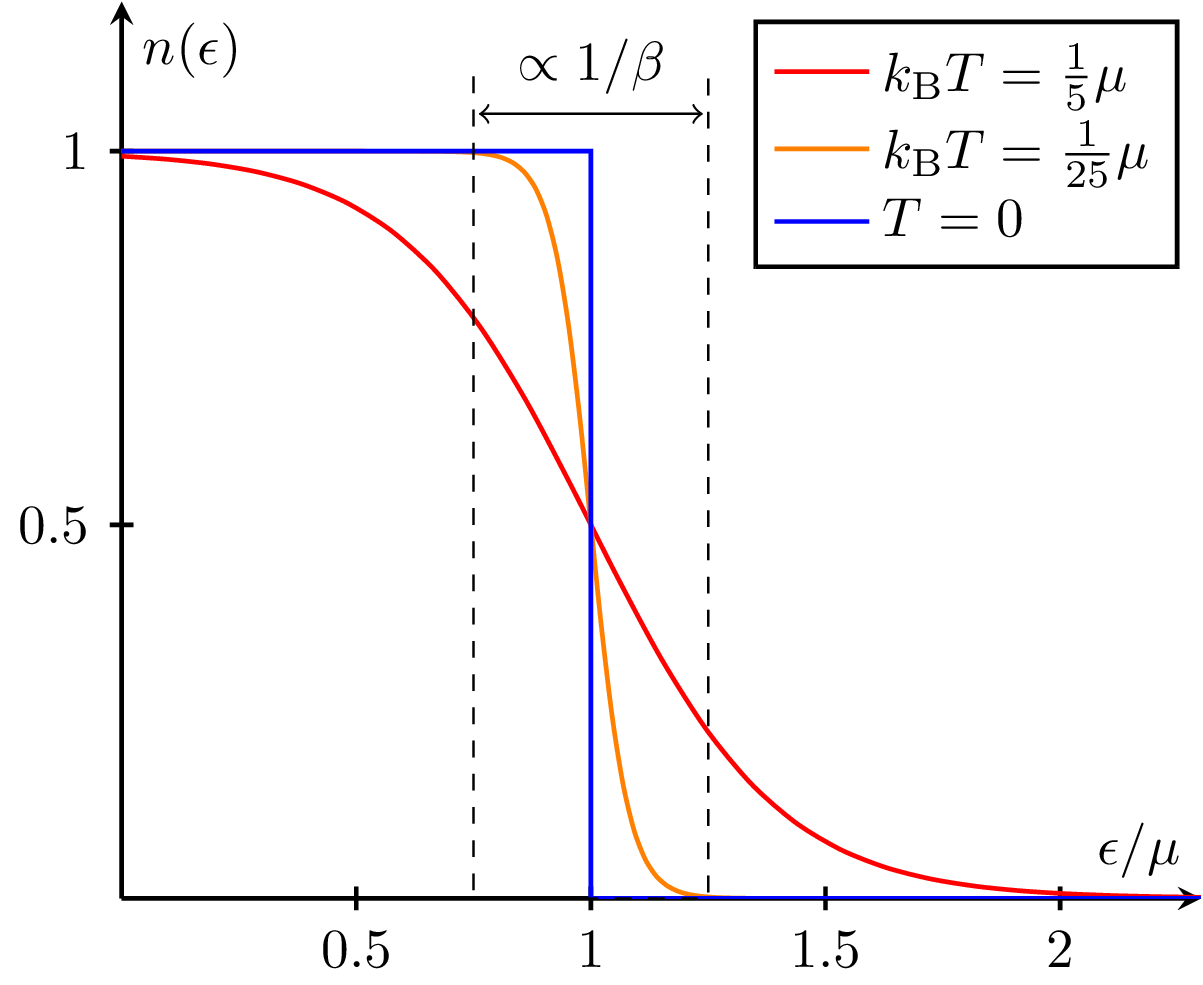
\includegraphics[width=0.3\linewidth]{fermidirac.png}
            \caption{Fermi-Dirac distribution for various temperatures.}
            \label{fig:fermidirac}
        \end{figure}

        Next, let us calculate the entropy.
        \begin{equation}
            S(k) = - \frac{\del \Phi_G}{\del T} = -\frac{\del \Phi_G}{\del \beta}\frac{d\beta}{dT}=k_B\beta^2 \frac{\del \Phi_G}{\del T}
        \end{equation}
        \begin{equation}
            \frac{\del \Phi_G}{\del \beta}=\frac{1}{\beta^2}\ln(1+e^{-\beta(\varepsilon-\mu)})+ \frac{1}{\beta}\frac{\varepsilon-\mu}{e^{\beta(\varepsilon-\mu)}+1}
        \end{equation}
        \begin{equation}
            \therefore S(k) = k_B\ln(1+e^{-\beta(\varepsilon-\mu)})+\frac{k_B\beta(\varepsilon-\mu)}{e^{\beta(\varepsilon-\mu)}+1}
        \end{equation}
        Now looking at the Fermi-Dirac distribution,
        \begin{equation}
            n(k) = \frac{1}{e^{\beta(\varepsilon-\mu)}+1}\implies e^{\beta(\varepsilon-\mu)}=\frac{1}{n}-1=\frac{1-n}{n}.
        \end{equation}
        Putting this into the entropy formula,
        \begin{align}
            S(k) =& k_B\ln\lrp{1+\frac{n}{1-n}}+\frac{k_B\ln\lrp{\frac{1-n}{n}}}{\frac{1-n}{n}+1}=k_B\ln\lrp{\frac{1}{1-n}}+nk_B\ln\frac{1-n}{n} \notag\\
                =& k_B\lrb{-\ln(1-n)+n\ln(1-n)-n\ln n} = -k_B[(1-n)\ln(1-n)+n\ln n]
        \end{align}
        This is the \textbf{fermionic entropy}. If $n(k)=0$, then $S(k)=0$ also if $n(k)=1$, $S(k)=0$. Since $n(k)=1$ at absolute zero, we can say that the Fermi gas at the absolute zero of temperature has no entropy. 
    
    \section{Bosons}
        Aforementioned system with bosons instead of fermions allow all occupations. 
        \begin{equation}
            \Theta(\v{k}) = 1+e^{-\beta(\varepsilon-\mu)}+e^{-2\beta(\varepsilon-\mu)}+\dots = \sum_{n=0}^{\infty}e^{-n\beta(\varepsilon-\mu)}
        \end{equation}    
        This is a geometric series:
        \begin{equation}
            \therefore \Theta(\v{k}) = \frac{1}{1-e^{-\beta(\varepsilon-\mu)}}.
        \end{equation}
        Then the grand potential is
        \begin{equation}
            \Phi_G = -k_BT\ln\Theta(\v{k}) = \frac{1}{\beta}\ln(1-e^{-\beta(\varepsilon-\mu)}).
        \end{equation}
        In calculating these, we utilised the geometric series sum. However, for that series to be convergent, the exponential must be less than unity and therefore $\varepsilon>\mu$. We will get to the implications of this later. If we calculate the average occupation in a similar manner as we did with the fermions, we obtain the \textbf{Bose-Einstein distribution}.
        \begin{equation}
            f(\v{k})=\frac{1}{e^{\beta(\varepsilon-\mu)}-1}
        \end{equation}
        Similar to Fermi-Dirac distribution, high temperature limit gives $e^{-\beta(\varepsilon-\mu)}$. Note that this is the Maxwell-Boltzmann distribution. Therefore, both the fermions and bosons obey the Maxwell-Boltzmann distribution at high temperatures. This is the classical limit of statistical thermodynamics. We will get to the low temperature limit later. The \textbf{bosonic entropy} is similar to the fermionic entropy.
        \begin{equation}
            S(k) = k_B[(1+f)\ln(1+f)-f\ln f]
        \end{equation}
        Note that if $f(k)=0$, then $S(k)=0$.

    \section{Fermi Gas}
        We start by trying to understand the behaviour of the chemical potential as a function of temperature. In that, we calculate the total number of particles, $N$, in terms of the chemical potential. 
        \begin{equation}
            N = 2\sum_v{k} e^{-\beta(\varepsilon(\v{k})-\mu)}
        \end{equation}
        Here, the factor of 2 comes from considering the spin of the fermions. As the discrete $\v{k}$ goes to $k$ in the continuum limit, we get
        \begin{equation}
            N = 2\int n(k)D(k)dk.
        \end{equation}
        In the integral, $n(k)$ are the occupied states while $D(k)dk$ are the available states. Letting $\varepsilon(k)=\frac{\hbar^2k^2}{2m}$,
        \begin{equation}
            N = 2\int_{0}^{\infty}\frac{Vk^2}{2\pi^2}\frac{1}{e^{\beta(\frac{\hbar^2k^2}{2m}-\mu)}+1}dk.
        \end{equation}
        Changing the variables as
        \begin{equation}
            x^2 \equiv \frac{\hbar^2k^2}{2mk_BT} \implies 2xdx = \frac{\hbar^2}{mk_BT}kdk\hspace{0.25cm},\hspace{0.25cm}k=\sqrt{\frac{2mk_BT}{\hbar^2}}x
        \end{equation}
        and 
        \begin{equation}
            \eta = \frac{\mu}{k_BT},
        \end{equation}
        we get
        \begin{equation}
            n = \frac{N}{V}=\frac{1}{\pi^2}\lrp{\frac{2mk_BT}{\hbar^2}}^{3/2}\int_{0}^{\infty}\frac{x^3}{e^{x^2-\eta}+1}dx.
        \end{equation}
        This integral is hard to solve and therefore we stop here and write the number density as a function of temperature. We then deal with the rest of the solution manually.
        \begin{equation}
            n = \frac{1}{\pi^2}\lrp{\frac{2mk_BT}{\hbar^2}}^{3/2}f(\eta)\implies \eta = f^{-1}\lrp{n\pi^2\lrp{\frac{\hbar^2}{2mk_BT}}^2}
        \end{equation}
        Now we look at the behaviour at absolute zero. Recall that the energy of a fermi gas at absolute zero was the Fermi energy. With this, we define the \textbf{Fermi wavevector}, $k_F$.
        \begin{equation}
            k_F = \frac{\sqrt{2mE_F}}{\hbar}
        \end{equation}
        We then find the Fermi wavevector in terms of $n=N/V$ using the constraint on $N$. For $k<k_F$, $n(k)=1$. Then,
        \begin{equation}
            N = 2\int_{0}^{\infty}n(k)D(k)dk = 2\int_{0}^{k_F}D(k)dk = \frac{2V}{2\pi^2}\int_{0}^{k_F}k^2dk = \frac{V}{\pi^2}\frac{k_F^3}{3}
        \end{equation}
        \begin{equation}
            \therefore k_F = (3n\pi^2)^{1/3}.
        \end{equation}
        Now, looking at the internal energy,
        \begin{equation}
            U = \frac{V}{\pi^2}\int_{0}^{k_F}k^2\lrp{\frac{\hbar^2k^2}{2m}}dk = \frac{V\hbar^2}{2m\pi^2}\frac{k_F^5}{5}=\underbrace{\frac{Vk_F^3}{3\pi^2}}_N\underbrace{\frac{\hbar^2k_F^2}{2m}}_{E_F}\frac{3}{5}=\frac{3N}{5}E_F
        \end{equation}
        So far, we considered only $\Phi_G(\v{k})$. To get the total grand potential, we integrate over $v{k}$.
        \begin{equation}
            \Phi_G = -\frac{Vk_BT}{\pi^2}\int_{0}^{\infty}k^2\ln(1+e^{-\beta(\varepsilon(k)-\mu)})dk = -\frac{Vk_BT}{\pi^2}\int_{0}^{\infty}k^2\ln(1+e^{-\beta(\frac{\hbar^2k^2}{2m}-\mu)})dk
        \end{equation}
        To reduce this integral to a familiar form, we use integration by parts. 
        \begin{equation}
            x^2 = \frac{\hbar^2k^2}{2m}\beta\implies k=\sqfrac{2mk_BT}{\hbar^2}x \hspace{0.25cm},\hspace{0.25cm} dk = \sqfrac{2mk_BT}{\hbar^2}dx
        \end{equation}
        \begin{equation}
            I = \lrp{\frac{2mk_BT}{\hbar^2}}^{3/2}\int x^2\ln(1+e^{-(x^2-\eta)})dx
        \end{equation}
        \begin{align}
            u = \ln(1+e^{-(x^2-\eta)}) \hspace{0.5cm}& du=\frac{-2xe^{-(x^2-\eta)}}{1+e^{-(x^2-\eta)}}=\frac{-2x}{e^{x^2-\eta}+1} \\
            dv = x^2dx \hspace{0.5cm}& v =\frac{x^3}{3}
        \end{align}
        \begin{equation}
            I = \bigg(\cdots\bigg)^{3/2}\lrb{\underbrace{\lrp{\frac{x^3}{3}\ln(1+e^{-(x^2-\eta)})}_0^\infty}_0+ \frac{2}{3}\int_{0}^{\infty}\frac{x^4}{e^{x^2-\eta}+1}dx}
        \end{equation}
        The pressure of the Fermi gas in terms of the total grand potential is
        \begin{equation}
            P = \frac{\Phi_G}{V}.
        \end{equation}
        Then, we get
        \begin{equation}
            P = \frac{2k_BT}{3\pi^2}\lrp{\frac{2mk_BT}{\hbar^2}}^{3/2}\int_{0}^{\infty}\frac{x^4}{e^{x^2-\eta}+1}dx.
        \end{equation}
        Now, let us see if we can derive an equivalent form of the ideal gas law. Starting from the density of particles and doing the same change of variables as before,
        \begin{equation}
            n = \frac{N}{V} = \frac{1}{V}\int_{0}^{\infty}D(k)n(k)dk = \frac{1}{\pi^2}\int_{0}^{\infty}\frac{k^2dk}{e^{\beta(\varepsilon-\mu)}+1}
        \end{equation}
        \begin{equation}
            n = \frac{1}{\pi^2}\lrp{\frac{2mk_BT}{\hbar^2}}^{3/2}\int_{0}^{\infty}\frac{x^2dx}{e^{x^2-\eta}+1}
        \end{equation}
        Combining this with the pressure expresion,
        \begin{equation}
            \frac{P}{nk_BT}=\frac{2}{3}\frac{\int_{0}^{\infty}\frac{x^4dx}{e^{x^2-\eta}+1}}{\int_{0}^{\infty}\frac{x^2dx}{e^{x^2-\eta}+1}}=\frac{2}{3}\frac{\frac{3}{8}\sqrt{\pi}}{\frac{1}{4}\sqrt{\pi}}=1 \implies PV = Nk_BT
        \end{equation}
        At absolute zero, we go back to the original expression.
        \begin{equation}
            P = \frac{k_BT}{\pi^2}\int_{0}^{\infty}k^2\ln(1+e^{-\beta(\varepsilon-\mu)})dk 
        \end{equation}
        Doing integration by parts,
        \begin{align}
            du = k^2 dk \hspace{0.5cm}& u = \frac{k^3}{3}\\
            v = \ln\lrp{1+e^{-\beta\lrp{\frac{\hbar^2k^2}{2m}-\mu}}} \hspace*{0.5cm}& dv = -\frac{\beta\hbar k}{m}\frac{e^{-\beta(\dots)}}{1+e^{-\beta(...)}}
        \end{align}
        The last factor in $dv$ is the Fermi-Dirac distribution which is 1 if $k<k_F$ and 0 if $k>k_F$ at absolute zero. Then,
        \begin{equation}
            P = \frac{k_BT}{\pi^2}\frac{\hbar^2}{mk_BT}\frac{1}{3}\int_{0}^{k_F}k^4dk = \frac{\hbar^2k_F^5}{15m\pi^2}=\frac{2}{5}\frac{\hbar^2k_F^2}{2m}\frac{k_F^3}{3\pi^2}
        \end{equation}
        \begin{equation}
            \therefore P = \frac{2nE_F}{5}
        \end{equation}
        This means that we have finite pressure at absolute zero. \\
        Finally, let us look at the low temperature behaviour of the Fermi gas. Defining the \textbf{Fermi temperature}, $T_F$, via $k_BT_F=E_F$; for temperature lower than the Fermi temperature, the gas is degenerate. The heat capacity at temperatures lower than the Fermi temperature is
        \begin{equation}
            C_V = \frac{Nk_B\pi^2}{2}\frac{k_BT}{E_F}.
        \end{equation}
        
    \section{Non-Interacting Bose Gas}
        While working with bosons, we will index over the energies rather than states since multiple particles can occupy the same state. We begin by defining a quantity called \textbf{fugacity}, $z=e^{\beta\mu}$. With fugacity, the average particle number is 
        \begin{equation}
            \expval{N} = \sum_\varepsilon\expval{n_\varepsilon} = \sum_\varepsilon\frac{1}{z^{-1}e^{\beta\varepsilon}-1}.
        \end{equation}
        We can convert this to an integral via
        \begin{equation}
            \expval{N} = \int D(\varepsilon)f(\varepsilon)d\varepsilon = \frac{Vm\sqrt{2m}}{2\pi^2\hbar^3}\int\frac{\sqrt{\varepsilon}}{z^{-1}e^{\beta\varepsilon}-1}d\varepsilon.
        \end{equation}
        However, note that $\varepsilon=0$ in the integral gives zero while it is nonzero in the sum. Therefore, we add $\varepsilon=0$ term by hand. We keep the lower limit on the integral still at zero since the integral is continous and not discrete as the sum.
        \begin{equation}\label{eq:bosestar}
            N = \frac{2\pi}{h^3}(2m)^{3/2}V\int_{0}^{\infty}\frac{\sqrt{\varepsilon}d\varepsilon}{z^{-1}e^{\beta\varepsilon}-1}+ \frac{z}{1-z}
        \end{equation}
        Let us make a change of variables and look at the integral only. 
        \begin{equation}
            x = \beta\varepsilon \implies I  = \int_{0}^{\infty}\frac{\sqrt{k_BTx}}{z^{-1}e^x-1}k_BTdx
        \end{equation}
        Placing this into (\ref{eq:bosestar}) and defining $N_0 = z/(1-z)$, 
        \begin{equation}
            \frac{N-N_0}{V} = \frac{2\pi}{h^3}(2mk_BT)^{3/2}\int_{0}^{\infty}\frac{\sqrt{x}dx}{z^{-1}e^x-1}=\frac{2}{\sqrt{\pi}}\frac{1}{\lambda_D^3}\int_{0}^{\infty}\frac{\sqrt{x}dx}{z^{-1}e^x-1}.
        \end{equation}
        To calculate this integral we define \textbf{Bose-Einstein Functions} as
        \begin{equation}
            g_\nu(z)=\frac{1}{\Gamma(\nu)}\int_{0}^{\infty}\frac{x^{\nu-1}dx}{z^{-1}e^x-1},
        \end{equation}
        where $\Gamma(\nu)$ is the gamma function. In our case, we have $g_{3/2}(z)$ with $\Gamma\lrp{\frac{3}{2}}=\frac{\sqrt{\pi}}{2}$. Then,
        \begin{equation}
            \frac{N-N_0}{V}=\frac{g_{3/2}(z)}{\lambda_D^3} =: \frac{N_e}{V}.
        \end{equation}
        Looking at the second term in (\ref{eq:bosestar}), 
        \begin{equation}
            N_0 = \frac{z}{1-z}\implies z = \frac{N_0}{1+N_0}.
        \end{equation}
        Therefore, $0\leq z \leq 1$. Then, when fugacity takes its maximum value, i.e. 1;
        \begin{equation}
            N_e = \frac{V}{\lambda_D^3}g_{3/2}(1).
        \end{equation}
        This value of the Bose-Einstein function is equal to the Riemann zeta function of 3/2. Also, $g_{3/2}(z)$ is a monotonic function. Therefore, if $z=1$ is the maximum fugacity, 
        \begin{equation}
            g_{3/2}(z)\leq \zeta\lrp{\frac{3}{2}}
        \end{equation}
        and 
        \begin{equation}
            N_e \leq \frac{V}{\lambda_D^3}\zeta\lrp{\frac{3}{2}}.
        \end{equation}
        This puts a limit to how many particles we may have in the system. Now a question is: What happens if we add more particles? In that case, excited states will take as many particles as they can while the remaining particles will be pushed to the ground state $\varepsilon=0$.
        \begin{equation}
            N_0 = N - \frac{V}{\lambda_D^3}\zeta\lrp{\frac{3}{2}}
        \end{equation}
        The value of $z$ is now determined by
        \begin{equation}
            z = \frac{N_0}{N_0+1}\approx 1 
        \end{equation}
        for large $N_0.$ This phenomenon of a very large number of particles occupying the same ground state is called the \textbf{Bose-Einstein condensation}. The transition temperature at which a Bose-Einstein condensate begins to form is found via 
        \begin{equation}
            N_e^\mathrm{max} = V\frac{(2\pi mk_BT_c)^{3/2}}{h^3}\zeta\lrp{\frac{3}{2}}.
        \end{equation}
        For $T<T_c$, the system is a mixture of two phases:
        \begin{itemize}
            \item[-] Normal phase with $N_e$ particles 
            \item[-] Condensed phase with $N_0=N-N_e$ particles.  
        \end{itemize}
        Now, let us look at the thermodynamical variables of a Bose gas. Starting with pressure,
        \begin{equation}
            P = -\frac{\del \Phi_G}{\del V} = -\frac{\Phi_G}{V}\implies PV=k_BT\ln\Theta \implies \beta PV=\ln\Theta.
        \end{equation}
        In the case of bosons with $T>T_c$:
        \begin{equation}
            \beta P = -\int_{0}^{\infty}\ln(1-ze^{-\beta\varepsilon})\underbrace{\frac{2\pi V}{h^3}(2m)^{3/2}\sqrt{\varepsilon}}_{D(\varepsilon)}d\varepsilon.
        \end{equation}
        Changing the variables and integrating by parts gives
        \begin{equation}
            \beta P = 2\pi\lrp{\frac{\sqrt{2mk_BT}}{h}}^3\frac{2}{3}\int_{0}^{\infty}\frac{x^{3/2}dx}{ze^{-x}-1}=\frac{1}{\lambda_D^3}g_{5/2}(z).
        \end{equation}
        For $T<T_c$, fugacity goes to unity and we get
        \begin{equation}
            \frac{P}{k_BT}=\frac{1}{\lambda_D^3}\zeta\lrp{\frac{5}{2}}.
        \end{equation}
        Now, looking at the internal energy,
        \begin{equation}
            U=-\frac{\del \ln\Theta}{\del \beta}=kT^2 \frac{\del }{\del T}\lrp{\frac{PV}{k_BT}}=k_BT^2Vg_{5/2}(z) \frac{\del \lambda_D^{-3}}{\del T}
        \end{equation}
\newpage
    \section{Exercises}
        \begin{eocproblem*}{}
            Using the continuous approximation, discuss the phenomenon of the Bose-Einstein condensation and the existence of a critical temperature for one and two dimensional systems with edge length $L$. Assume $\varepsilon=p^2/2m$.
        \end{eocproblem*}
            Here we need to work through the occupation number for each dimension. Starting with two dimensions, 
            \begin{equation}
                D_2(\varepsilon) = \frac{A m}{2\pi\hbar^2}.
            \end{equation}
            \begin{equation}
                \implies \expval{N} = \int \frac{A m}{2\pi\hbar^2}\frac{1}{e^{\beta(\varepsilon-\mu)}-1}d\varepsilon
            \end{equation}
            Substituting $x=\beta\varepsilon$,
            \begin{equation}
                \expval{N} = k_BT\frac{A m}{2\pi\hbar^2}\int \frac{dx}{e^{x-\beta\mu}-1} = k_BT\frac{Am}{2\pi\hbar^2}\int\frac{dx}{z^{-1e^x-1}}
            \end{equation}
            At critical temperature, $\mu\to0$.
            \begin{equation}
                \therefore \expval{N} = k_BT_c\frac{Am}{2\pi\hbar^2}\int\frac{dx}{e^x-1} = k_BT_c\frac{Am}{2\pi\hbar^2}\zeta(1)
            \end{equation}
            Since zeta function at $x=1$ is divergent, the occupation number diverges at critical temperatures in two dimensions.\\
            Now consider one dimension. 
            \begin{equation}
                \expval{N} = \frac{L\sqrt{m}}{\sqrt{2}\pi\hbar^2}\int\varepsilon^{-1/2}\frac{d\varepsilon}{e^{\beta(\varepsilon-\mu)}-1}
            \end{equation}
            Again, substituting $x=\beta\varepsilon$,
            \begin{equation}
                \expval{N} = \frac{L\sqrt{m}}{\pi\hbar^2\sqrt{2}}\int(k_BTx)^{-1/2}\frac{k_BT dx}{e^{x-\eta}-1}.
            \end{equation} 
            \begin{equation}
                \expval{N} = \frac{L}{\pi\hbar^2}\sqfrac{mk_BT}{2}\int\frac{x^{-1/2}dx}{z^{-1}e^x-1} = \frac{L}{\pi\hbar^2}\sqfrac{mk_BT}{2}g_{1/2}(z).
            \end{equation}
            Again, at critical temperature, we get a zeta divergence. Thus in both cases $T_c=0$ and there is no Bose-Einstein condensation.
        \begin{eocproblem*}{}
            Consider a collection of $\expval{N}$ bosonic quantum harmonic oscillators in two dimensions with spin-0 and frequency $\omega$.
            \begin{enumerate}
                \item[i)] Identify the critical value of the chemical potential $\mu_c$ for which the $\expval{N}$ has a divergence.
                \item[ii)] Give an estimate for the chemical potential $\mu$ in the limit $z\to0$. 
                \item[iii)] Discuss the existence of a Bose-Einstein condensate.   
            \end{enumerate}
        \end{eocproblem*}
            \paragraph{i)}
            The average particle number for a state with quantum numbers $(n_x,n_y)$ is
            \begin{equation}
                \bar{n}(n_x,n_y) = \frac{1}{z^{-1}e^{\beta\hbar\omega(n_x+n_y+1)}-1}.
            \end{equation}
            To find the total average number of particles, we convert the double sum to a single sum: $n_x+n_y=n$. Then for each $n_x=0,...,n$ there is one $n_y=n-n_x$. This means that there are $n+1$ possible combinations. Thus, 
            \begin{equation}
                \expval{N} = \sum_{n=0}^{\infty}\frac{n+1}{z^{-1}e^{\beta\hbar\omega(n+1)}-1}.
            \end{equation} 
            For $\expval{N}$ to be divergent, $z^{-1}e^{\beta\hbar\omega(n+1)}-1$=0. Then at the ground state,
            \begin{equation}
                z_c = e^{\beta\hbar\omega} \implies \mu_c = \hbar\omega.
            \end{equation}
            \paragraph{ii)} As $z\to0$, the denominator will grop rapidly and therefore we can neglect the $-1$ term. Then, $\expval{N}$ can be approximated by
            \begin{equation}
                \expval{N} = \sum_{n_x,n_y=0}^{\infty}\frac{1}{z^{-1}e^{\beta\hbar\omega(n_x+n_y+1)}-1}\approx ze^{\beta\hbar\omega}\sum_{n_x,n_y=0}^{\infty}e^{-\beta\hbar\omega(n_x+n_y)}.
            \end{equation}
            In this case, the $n_x$ and $n_y$ are independent. Thus,
            \begin{equation}
                \expval{N} \approx ze^{\beta\hbar\omega}\lrp{\sum_{n=0}^{\infty}e^{-n\beta\hbar\omega}}^2=\frac{ze^{-\beta\hbar\omega}}{(1-e^{-\beta\hbar\omega})^2}=\frac{z}{4\sinh^2\frac{\beta\hbar\omega}{2}}.
            \end{equation}
            This gives the chemical potential as
            \begin{equation}
                \mu = \frac{1}{\beta}\ln\lrp{4\expval{N}\sinh^2\frac{\beta\hbar\omega}{2}}.
            \end{equation}
            \paragraph{iii)} The critical temperature is found by imposing $\mu\to\mu_c$, $T=T_c$, $N=0$.
            \begin{equation}
                \expval{N} = \sum_{n=1}^{\infty}\frac{n+1}{e^{n\beta_c\hbar\omega}-1}
            \end{equation}
\newpage
        \begin{eocproblem*}{}
            Compute the average number of particles for a fully degenerate relativistic gas with $s=1/2$ in a cubic container of edge length $L$. The gas is under the effect of a constant gravitational acceleration $g$ acting along one direction. Consider explicitly the cases
            \begin{enumerate}
                \item[i)] Non-relativistic: $v<<c$
                \item[ii)] Ultrarelativistic: $v\approx c$ 
            \end{enumerate}
        \end{eocproblem*}
            General expression for the momentum is
            \begin{equation}
                \v{p} = \frac{m\v{v}}{\sqrt{1-\frac{v^2}{c^2}}}
            \end{equation}
            with
            \begin{equation}
                \varepsilon_k(p) = c\sqrt{p^2+m^2c^2}.
            \end{equation}
            For non-relativistic case, the kinetic energy $\varepsilon_k = p^2/2m$ while for ultrarelativistic case $\varepsilon_k=pc$. Then, the total energies are $\varepsilon = \frac{p^2}{2m}+mgx$ and $\varepsilon=pc+mgx$ respectively. Now, we are to find $\expval{N}$ in terms of $\varepsilon_F$ at $T=0$. For the non-relativistic case,
            \begin{equation}
                \expval{N} = \frac{4\pi(2s+1)}{(2\pi\hbar)^3}L^3\int_{0}^{\sqrt{2m\varepsilon_F}}p^2dp\int_{0}^{-\frac{p^2}{2m^2g}+\frac{\varepsilon_F}{mg}}dx = \frac{L^2}{\pi^2\hbar^3}\frac{4\sqrt{2}}{15}\frac{\varepsilon_F^{5/2}\sqrt{m}}{g}.
            \end{equation}
            For the ultrarelativistic case,
            \begin{equation}
                \expval{N} = \frac{L^2}{\pi^2\hbar^3}\int_{0}^{\varepsilon_F/c}p^2dp\int_{0}^{\frac{-pc+\varepsilon_F}{mg}}dx=\frac{L^2}{\pi^2\hbar^3}\frac{\varepsilon_F^4}{12mgc^3}.
            \end{equation}
        \begin{eocproblem*}{}
            An average number $N$ of fermions is placed in a volume $V$ at temperature $T=0$. The single particle energy is $\varepsilon=\frac{p^2}{2m}$. Give an estimate for the isothermal compressibility
            \begin{equation}
                K_T = -\frac{1}{V}\lrp{\frac{\del V}{\del P}}_{T,N}.
            \end{equation}

        \end{eocproblem*}
            At $T=0$, $F=U-TS=U$. Moreover, we know that the pressure is
            \begin{equation}
                P=\frac{2n\varepsilon_F}{5}=\frac{2n}{5}\frac{5U}{3N} \implies U = \frac{3}{5}N\varepsilon_F\implies \varepsilon_F = \frac{5U}{3N}.
            \end{equation}
            Then, $PV = 2U/3$. 
            \begin{equation}
                P = -\frac{\del F}{\del V} = -\frac{\del U}{\del V} = -\frac{\del }{\del V}\lrp{\frac{2}{3}PV}=-\frac{2}{3}\lrp{V \frac{\del P}{\del V}+P}
            \end{equation}
            Evaluating the first term with $\varepsilon_F = \frac{\hbar^2k_F^2}{2m}=\frac{\hbar^2}{2m}(3\pi^2N)^{2/3}$,
            \begin{equation}
                \frac{\del P}{\del V} = \frac{\del }{\del V}\lrp{\frac{2N}{5}\frac{\hbar^2}{2m}(3\pi^2N)^{2/3}} = \frac{3\pi^2\hbar^2}{2m}\frac{2}{5} \frac{\del }{\del V}\lrp{\frac{N}{V}}^{5/3}.
            \end{equation}
            \begin{equation}
                \therefore V \frac{\del P}{\del V}=\frac{5}{3}P = \frac{10U}{9V}
            \end{equation}
            \begin{equation}
                \therefore K = -\frac{1}{V} \frac{\del V}{\del P}=\lrp{\frac{\hbar^2}{3m}(3\pi^2)^{2/3}\lrp{\frac{N}{V}^{5/3}}}^{-1}
            \end{equation}